%%%%%%%%%%%%%%%%%%%%%%%%%%%%%%%%%%%%%%%%%%%%%%%%%%%%%%%%%%%%%%%%%%%%%
% PREAMBLE
%%%%%%%%%%%%%%%%%%%%%%%%%%%%%%%%%%%%%%%%%%%%%%%%%%%%%%%%%%%%%%%%%%%%%
%
% The following two commands will generate a PDF that follows all the requirements for submission
% and peer review.  Uncomment these commands to generate this output (and comment out the two lines below.)
%
% DOUBLE SPACE VERSION FOR SUBMISSION TO THE AMS
%\documentclass[12pt]{article}
%\usepackage{ametsoc}
%\linenumbers
%
% The following two commands will generate a single space, double column paper that closely
% matches an AMS journal page.  Uncomment these commands to generate this output (and comment
% out the two lines above. FOR AUTHOR USE ONLY. PAPERS SUBMITTED IN THIS FORMAT WILL BE RETURNED
% TO THE AUTHOR for submission with the correct formatting.
%
% TWO COLUMN JOURNAL PAGE LAYOUT FOR AUTHOR USE ONLY
\documentclass[10pt]{article}
\usepackage{ametsoc2col}
%\usepackage{dblfloatfix}

%
%%%%%%%%%%%%%%%%%%%%%%%%%%%%%%%%%%%%%%%%%%%%%%%%%%%%%%%%%%%%%%%%%%%%%
% ABSTRACT
%
% Enter your Abstract here
%%%%%%%%%%%%%%%%%%%%%%%%%%%%%%%%%%%%%%%%%%%%%%%%%%%%%%%%%%%%%%%%%%%%%
\newcommand{\myabstract}{We develop a technique for smoothing noisy GPS data using B-splines with tension. We show how the tension condition routinely employed in smoothing splines can be restated as a maximum likelihood problem and then how the tension parameter can be chosen based on physical reasoning. The GPS errors appear to be non-Gaussian, so we use a t-distribution in the maximum likelihood.  }
%
\begin{document}
%
%%%%%%%%%%%%%%%%%%%%%%%%%%%%%%%%%%%%%%%%%%%%%%%%%%%%%%%%%%%%%%%%%%%%%
% TITLE
%
% Enter your TITLE here
%%%%%%%%%%%%%%%%%%%%%%%%%%%%%%%%%%%%%%%%%%%%%%%%%%%%%%%%%%%%%%%%%%%%%
\title{\textbf{\large{Smoothing Noisy GPS Data with Tension}}}
%
% Author names, with corresponding author information. 
% [Update and move the \thanks{...} block as appropriate.]
%
\author{\textsc{J. J. Early,}
				\thanks{\textit{Corresponding author address:} 
				Jeffrey J. Early, NorthWest Research Associates, 
				4118 148th Ave NE, Redmond, WA 98052. 
				\newline{E-mail: jearly@nwra.com}}\quad\textsc{A. Sykulski}\\
}
%
% Formatting done here...Authors should skip over this.  See above for abstract.
\ifthenelse{\boolean{dc}}
{
\twocolumn[
\begin{@twocolumnfalse}
\amstitle

% Start Abstract (Enter your Abstract above.  Do not enter any text here)
\begin{center}
\begin{minipage}{13.0cm}
\begin{abstract}
	\myabstract
	\newline
	\begin{center}
		\rule{38mm}{0.2mm}
	\end{center}
\end{abstract}
\end{minipage}
\end{center}
\end{@twocolumnfalse}
]
}
{
\amstitle
\begin{abstract}
\myabstract
\end{abstract}
\newpage
}
%%%%%%%%%%%%%%%%%%%%%%%%%%%%%%%%%%%%%%%%%%%%%%%%%%%%%%%%%%%%%%%%%%%%%
% MAIN BODY OF PAPER
%%%%%%%%%%%%%%%%%%%%%%%%%%%%%%%%%%%%%%%%%%%%%%%%%%%%%%%%%%%%%%%%%%%%%
\section{Introduction}
Global positioning system receivers (now commonly referred to as `a GPS') are used in literally billions of devices around the the world to track positions. The quality of the position data can be quite good, with accuracies down to a few meters (cite gps.gov), but real world effects (such as atmospheric conditions sky blockages, to quote gps.gov) can significantly increase the errors. Kalman filters are often employed to reduce these errors because they can be run in real time (cite something). Here we consider an alternative approach using smoothing B-splines to control errors for data that has been collected and archived.

The data shown here was collected from from oceanic surface \emph{drifters}, floating buoys with drogues tethered 15-30 meters below the ocean surface, depending on the particular experiment. In the past, these drifters have used Argos positioning system which has significantly poorer temporal coverage and position accuracy (cite elipot), but recently more surface drifters have employed GPS receivers and transmitted their data back through Argos or Iridium satellites. The GPS receiver sits on the surface buoy and collects position data, but because of atmospheric conditions or ocean waves, the receivers are sometimes unable to obtain a position, or when they do, it is highly inaccurately. Thus, despite nominal accuracies of a few meters, it is often the case that some data is off by more than 1000 meters.

In addition to correcting the position errors, it is also important to interpolate the data to a regular grid. Although the sampling period of a GPS receiver can be fixed, because of missing data and time to to acquire signals, the sampling can be quite irregular. Because many analysis techniques require regular sampling (e.g., a Fourier transform), it is necessary to interpolate the signal onto a regular grid. So the approach taken here is not to simply discard poor data, but also to interpolate the position.

For this particular note we will consider nine surface drifters that were deployed in the Sargasso Sea in the summer of 2011. These particular drifters were part of the LatMix experiment (cite BAMs) and recorded data at approximately 30 minute intervals over the course of a week before being retrieved.

%%%%%%%%%%%%%%%%%%%%%%
%
\section{Maximum Likelihood}
%
%%%%%%%%%%%%%%%%%%%%%%

Throughout this discussion assume that we have collected bivariate time series data of drifter positions given as either projected coordinates $(x_i, y_i)$ or longitude/latitude $(\phi_i, \theta_i$) at times $t_i$. The goal is to create a model of position $(x(t),y(t))$ that is continuous in $t$, and perhaps even continuous a higher derivative---such as velocity or acceleration---that best matches the data given an assumed set of errors.

Slightly rewording a quote from Numerical Recipes, the central idea of maximum likelihood is to ask ``Given a particular path $(x(t),y(t))$, what is the probability that this dataset $(t_i,x_i, y_i)$ could have occurred?'' The goal is then to find the path that is most likely to have produced that dataset.

Conceptually we have two major pieces that we need to solve this problem:
\begin{enumerate}
\item we need to specify the probability function and
\item we need to specify the form of the path (model).
\end{enumerate}

%%%%%%%%%%%%%%%%%%%%%%
\subsection{Gaussian errors}
%%%%%%%%%%%%%%%%%%%%%%

The probability function is used to describe the errors in the position, $\epsilon_i \equiv x_i - x(t_i)$. The canonical example in one-dimension is to assume that the error in our position measurements are Gaussian and therefore the probability of the observed data given the model is,
\begin{equation}
\label{max-gaussian}
P \sim \prod \exp \left[ -\frac{1}{2} \left( \frac{x_i - x(t_i)}{\sigma_i} \right)^2 \right] \Delta x
\end{equation}
where $x_i$ represents the observations at time $t_i$ with estimated error of $\sigma_i$.

Maximizing the probability function in equation \ref{max-gaussian} is also the same as minimizing its argument (called the penalty function),
\begin{equation}
\label{least-squares}
\phi = \sum \left[\frac{1}{2} \left( \frac{x_i - x(t_i)}{\sigma_i} \right)^2 \right].
\end{equation}
Stated in this way is plain to see that this is the same as asking for the `least-squares' fit of the errors.

%%%%%%%%%%%%%%%%%%%%%%
\subsection{A model}
%%%%%%%%%%%%%%%%%%%%%%

Simply connecting a straight line to each individual data point would certainly maximize equation \ref{max-gaussian} (and minimize equation least-squares) because it would set all the errors to zero, but the resulting distribution of errors (a delta function at zero) wouldn't look anything like the assumed Gaussian distribution. Thus, if we want the error distribution that we get out to look like that which we assumed, it also necessary to \emph{constrain} the problem in some way. There are conceptually (at least) two ways of doing this, either 
\begin{enumerate}
\item specify a model with fewer degrees of freedom than data points, or
\item specify an additional \emph{global} constraints on the model in the penalty function.
\end{enumerate}
These two may be equivalent. For example, you may decide the model is a straight line (with two degrees of freedom), or you could set a constraint that that the integral of the second derivative vanish.

The approach taken h


%%%%%%%%%%%%%%%%%%%%%%
%
\section{B-Splines}
%
%%%%%%%%%%%%%%%%%%%%%%

A B-spline, or basis spline, of order $K$ is a piecewise polynomial function defined with respect to knot points. The terminology here is confusing, but generally seems to be that a B-spline of \emph{order} $K$, is a piecewise polynomial of \emph{degree} $S=K-1$. That means that a $4$th order B-spline is a piecewise cubic polynomial. The \emph{knot points} define the location where the polynomials meet. Continuity is maintained to as high of order as possible. For example, a $K=1$ B-spline is a piecewise constant function with value $1$ between two knot points, while $K=2$ B-spline forms a continuous triangle function with a piecewise constant first derivative (see figure \ref{bsplines}).

\begin{figure}[t]
  \noindent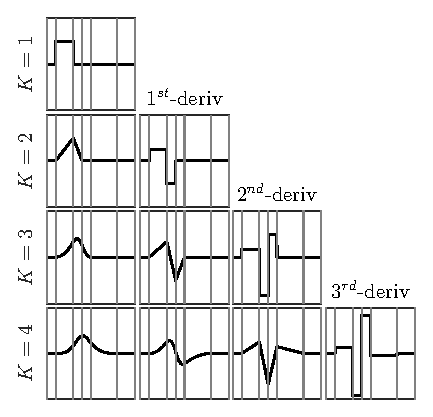
\includegraphics[width=19pc,angle=0]{bsplines}\\
  \caption{This shows an example B-spline and its derivatives (columns) for orders $K=1..4$ (rows).}
  \label{bsplines}
\end{figure}

%%%%%%%%%%%%%%%%%%%%%%
%
\section{Smoothing Spline}
%
%%%%%%%%%%%%%%%%%%%%%%


%\begin{acknowledgment} 
%Start acknowledgments here.
%\end{acknowledgment}
%
%% Use appendix}[A], {appendix}[B], etc. etc. in place of appendix if you have multiple appendixes.
%\ifthenelse{\boolean{dc}}
%{}
%{\clearpage}
%\begin{appendix}
%\section*{\begin{center}Appendix Title Is Entered Here (Primary heading)\end{center}}
%\subsection{First appendix secondary heading}
%
%\subsection{Second appendix secondary heading}
%
%\subsubsection{First appendix tertiary heading}
%
%\subsubsection{Second appendix tertiary heading}
%
%\paragraph{First appendix quaternary heading}
%
%\paragraph{Second appendix quaternary heading}
%
%\end{appendix}
%
%% Create a bibliography directory and place your .bib file there.
%% -REMOVE ALL DIRECTORY PATHS TO REFERENCE FILES BEFORE SUBMITTING TO THE AMS FOR PEER REVIEW
%\ifthenelse{\boolean{dc}}
%{}
%{\clearpage}
%\bibliographystyle{ametsoc}
%\bibliography{references}
%
%%%%%%%%%%%%%%%%%%%%%%%%%%%%%%%%%%%%%%%%%%%%%%%%%%%%%%%%%%%%%%%%%%%%%%
%% FIGURES-REMOVE ALL DIRECTORY PATHS TO FIGURE FILES BEFORE SUBMITTING TO THE AMS FOR PEER REVIEW
%%%%%%%%%%%%%%%%%%%%%%%%%%%%%%%%%%%%%%%%%%%%%%%%%%%%%%%%%%%%%%%%%%%%%%
%\begin{figure}[t]
%  \noindent\includegraphics[width=19pc,angle=0]{figure01.pdf}\\
%  \caption{Enter the caption for your figure here.  Repeat as
%  necessary for each of your figures. Figure from \protect\cite{Knutti2008}.}\label{f1}
%\end{figure}
%%%%%%%%%%%%%%%%%%%%%%%%%%%%%%%%%%%%%%%%%%%%%%%%%%%%%%%%%%%%%%%%%%%%%%
%% TABLES
%%%%%%%%%%%%%%%%%%%%%%%%%%%%%%%%%%%%%%%%%%%%%%%%%%%%%%%%%%%%%%%%%%%%%%
%\begin{table}[t]
%\caption{This is a sample table caption and table layout.  Enter as many tables as
%  necessary at the end of your manuscript. Table from Lorenz (1963).}\label{t1}
%\begin{center}
%\begin{tabular}{ccccrrcrc}
%\hline\hline
%$N$ & $X$ & $Y$ & $Z$\\
%\hline
% 0000 & 0000 & 0010 & 0000 \\
% 0005 & 0004 & 0012 & 0000 \\
% 0010 & 0009 & 0020 & 0000 \\
% 0015 & 0016 & 0036 & 0002 \\
% 0020 & 0030 & 0066 & 0007 \\
% 0025 & 0054 & 0115 & 0024 \\
%\hline
%\end{tabular}
%\end{center}
%\end{table}
%
\end{document}